\section{Diseño del hardware} 
Para el voltímetro se realizó una división tensiones \cite{electronics-stackexchange} como se observa en la figura \ref{hardware}, puesto que se necesita reducir el rango de tensiones al rango admitido por el Arduino UNO.


\begin{figure} [H]
    \centering
    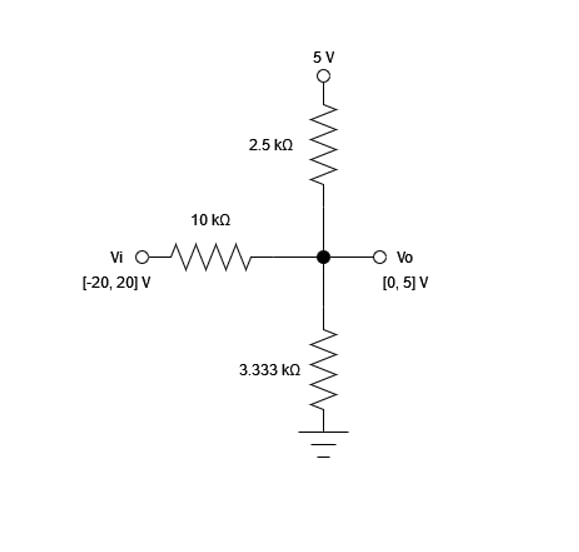
\includegraphics[width=11cm]{Imagenes/Hardware.jpg}
    \caption{Diseño de hardware para el voltímetro. Fuente y créditos: \cite{electronics-stackexchange}.}
    \label{hardware}
\end{figure}

Una vez que se realizó el diseño del divisor de tensiones, se realizó un diseño de un esquemático con la conexión de todos los componentes, y el circuitos anterior, como se muestra en la siguiente imagen.

\begin{figure} [H]
    \centering
    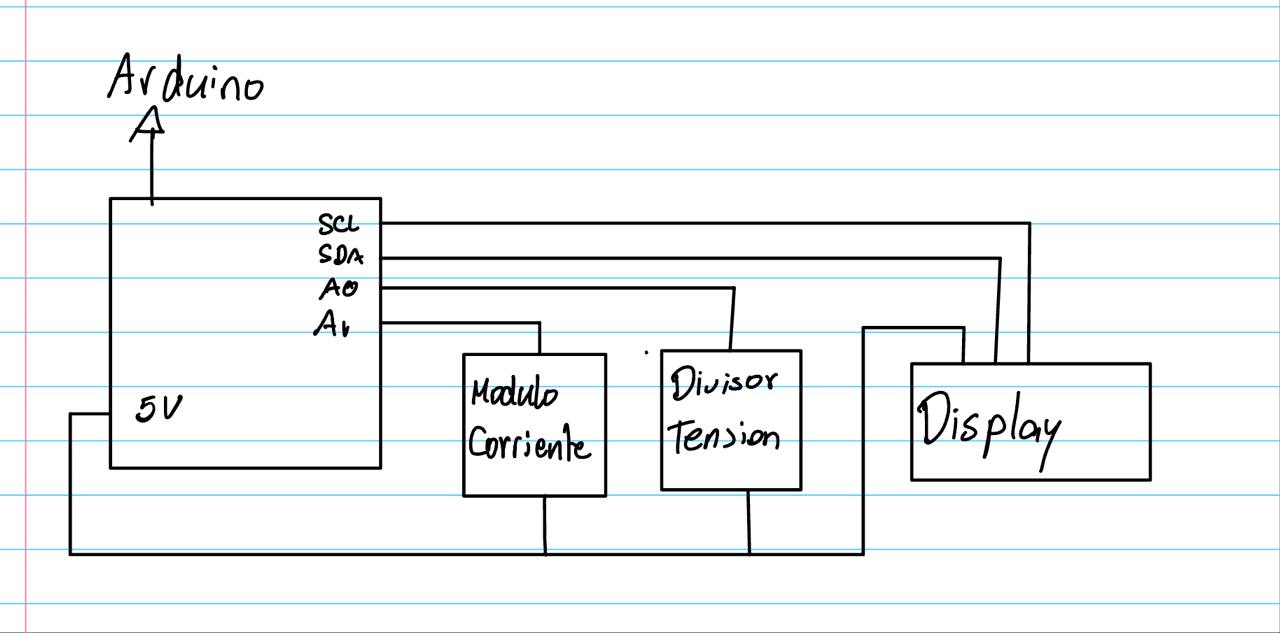
\includegraphics[width=11cm]{Imagenes/Esquematico.jpg}
    \caption{Esquemático del proyecto.}
    \label{Esquematico}
\end{figure}

